\documentclass[12pt,letterpaper,noanswers]{exam}
%\usepackage{color}
\usepackage[usenames,dvipsnames,svgnames,table]{xcolor}
\usepackage[margin=0.9in]{geometry}
\renewcommand{\familydefault}{\sfdefault}
\usepackage{multicol}
\pagestyle{head}
\usepackage{hyperref}
\usepackage[numbered,autolinebreaks,useliterate]{mcode}
\newcommand{\mb}[1]{\underline{#1}}

\header{AM 22b Problem Set 10}{}{Due Thurs Apr 29 at 6pm ET}
\runningheadrule
\headrule
\usepackage{diagbox}
\usepackage{graphicx} % more modern
%\usepackage{subfigure} 
\usepackage{amsmath} 
\usepackage{amssymb} 
%\usepackage{gensymb} 
%\usepackage{natbib}
\usepackage{hyperref}
%\usepackage{enumitem}
%\setlength{\parindent}{0pt}
%\usepackage{setspace}
%\pagestyle{empty}  
%\newcommand{\Sc}[0]{
%{\color{BlueViolet}\S}
%}
\usepackage{tcolorbox}

\begin{document}
 \pdfpageheight 11in 
  \pdfpagewidth 8.5in
 
\begin{questions}
\question Log in to WeBWorK and complete the problems assigned there under pset10.

\question (Toricelli's law)


There are a number of videos on \texttt{youtube} of Toricelli's law in action.  There is one in the problem set folder, downloaded in 2020 from \url{https://www.youtube.com/watch?v=TkVXObpcRAU}.

From the video, it is possible to extract the height of the water column as a function of time.

\begin{parts}
\item Use the matlab code that has been provided, along with the zipfile of images from the movie to extract a time series.
\item See the class handout from Class 33 for the derivation of the differential equation in the case of a draining cylinder.  

Write out a solution here for $\dfrac{dy}{dt} = -k y^{1/2}, y(0) = y_0$, including the time range over which the solution applies.  \emph{You can copy this from your work on the jamboard.}
\item In the matlab code, you'll fit this model (the solution expression for $y(t)$) to the data.  Revise the model in \texttt{fittype} to reflect your solution above.  \emph{I believe this will require the curve-fitting toolbox: remember that the online version of Matlab has all of the toolboxes}.

Run the curve fitting routine on different amounts of data and fill out a table similar to the one below.

\begin{tabular}{|c| c| c|c|c|}
\hline
frames in fit & fit value of $k$ & fit value of $y_0$ & predicted emptying time & how good is the fit?\\
\hline
1 - (5-10) & & & & \\
\hline
1 - (20-30) & & & & \\
\hline
1 - (45-50) & & & & \\
\hline
1 - 57 (all) & & & & \\
\hline
\end{tabular}
\part Towards the end of the video, the liquid appears to have finished draining, but the height of the liquid is not zero.  Add a parameter to your model to account for the fact that the liquid drains to a value $y_f$, rather than to zero, and redo your fit (use all of the data for this fit).  Provide the information in the table above, as well as the fit value of $y_f$.
\part Assuming that the container has a four inch diameter, and that drainage is through a circular hole, use $k$ to estimate the effective radius or diameter of the hole.  \emph{Be careful of units: $g$ should be in inches per second squared, or you'll need to convert all distances to meters.}
\part This is a differential equations model in a physics context.  We have also built simple models of population growth curves (US Census data).  

The world around us is complex.  In a model, we attempt to use mathematics to represent some aspect of the world in a more simple way.
\begin{itemize}
\itemsep0em
    \item We can use models to describe information in a compressed way (a single differential equation vs a list of data).
    \item We can use models to make predictions in forward time.
    \item We can use models to build strategies for designing and controlling systems.
\end{itemize}

In this physics context and in the population context, what is the value of building a model?  In each context, to what extent does a model fit on a portion of the data predict the future behavior of the system?
\end{parts}

\question (differential equations)
\begin{parts}
\item Find a solution to the initial value problem $\dfrac{dy}{dt} = ye^t, y(0) = 2e$
%\item Find a general solution to $t\dot y + (2t-3)y = 4t^4$.
\item For $\ddot x + 3 \dot x - 4x = 0$:
% \dot x = y
% \dot y = 4x-3y
\begin{itemize}
\itemsep0em
\item Write it as a first order system and find the matrix $A$ associated with its matrix form.  
    \item Compute the eigenvalues and eigenvectors of $A$ to generate a solution of the form $c_1\underline v_1e^{\lambda_1 t} + c_2 \underline v_2e^{\lambda_2 t}$.
    \item Use your solution to the first order system to write a solution $x(t)$ for the original second order differential equation.
    \item Verify that your $x(t)$ expression is a solution to the original second order differential equation.  \emph{Plug it into the left hand side of the equation and show that it simplifies to zero, so satisfied the equation.}
\end{itemize}
\item Toricelli's law states that $\dfrac{dV}{dt} = - c\sqrt{h}$, where $h$ is the height of the water in the container.  Construct a differential equation for when the shape of the outside of the container that is emptying is given by the paraboloid $z = x^2+y^2$.  If possible using the methods of our course, solve this differential equation with $h(0) = 4$ and give an expression for the emptying time.
\end{parts}

\question For each of the following systems of differential equations, 
\begin{itemize}
\itemsep0em
    \item Find the equilibrium solutions for the system (these are points $(x,y)$ where $\dot x$ and $\dot y$ are simultaneously zero).
    \item Match the system to one of the phase portraits shown (use the row and column of the portrait to specify it)
    \item Describe the behavior of the system along one flow line.
\end{itemize} 
\begin{parts}
\part $\dot x = x-y, \dot y = x+3y-4$
%\part $\dot x = x-2y +3, \dot y = x -y+2$
\part $\dot x = 1-y^2, \dot y = x+2y$
%\part $\dot x = 2-4x-15y, \dot y = 4-x^2$
\part $\dot x = x-2y, \dot y = 4x-x^3$
\part $\dot x = x-y-x^2+xy, \dot y = -y-x^2$
\end{parts}

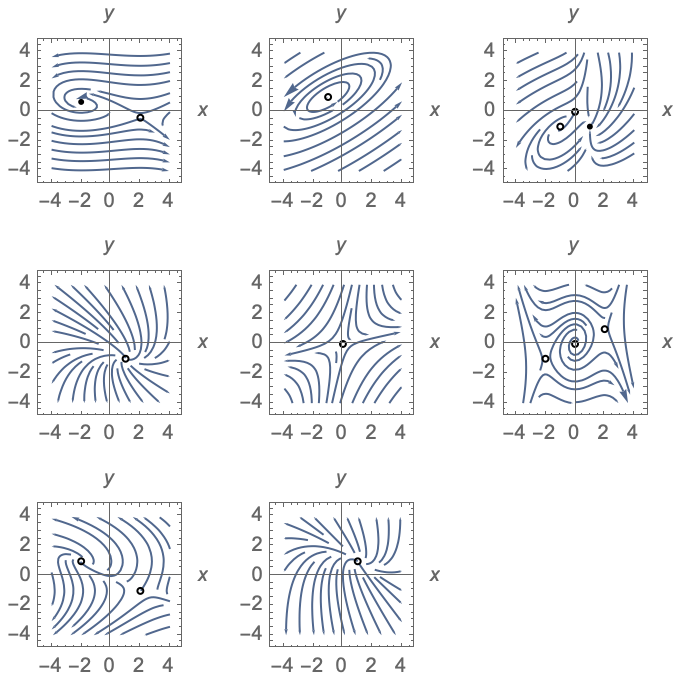
\includegraphics{img/S20pset10p1.png}

% \question 

% \begin{parts}
% \part Let $\underline F = F_1\underline i + F_2\underline j$ with $\partial_x F_2 - \partial_y F_1 = 3(x^2+y^2) - (x^2+y^2)^{3/2}$.  Let $C_a$ be the circle of radius $a$ in the $xy$-plane, centered at the origin and oriented counterclockwise.  For what value of $a$ is the line integral $\displaystyle\int_{C_a} \underline F \cdot d\underline r$ largest?
% \part Let $\underline F = \langle -y/r^2, x/r^2\rangle$ where $r^2 = x^2+y^2$.  $\underline F$ has zero curl where the vector field is defined (but it is not defined at $r = 0$).  For $C_1$ and $C_2$ the oriented curves shown in the figure below, show that $\displaystyle\int_{C_1}\underline F\cdot d\underline r = \int_{C_2}\underline F\cdot d\underline r  = \theta$, where $\theta$ is the angle at the origin subtended by the oriented curve $C_1$.

% 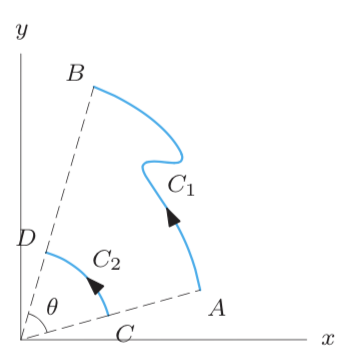
\includegraphics[scale=0.7]{img/S20pset10curl.png}
% \end{parts}


% \question diff eqs: separable, linear, 
% Consider the second order, linear, homogeneous differential equation $\ddot x - x = 0$.
% \begin{parts}
% \item Show that $x_1(t) = e^t$ is a solution to the differential equation. 
% \item   Rewrite this as a first order system in matrix form. 
% \item  Find the vector solution $\underline x = \left(\begin{array}{c} x \\ y\end{array}\right)$ for the solution above.
% \item $x_2(t) = e^{-t}$ is a second solution to the second order diff eq.  
% \end{parts}


% \question 
% The number of people who have been infected with a disease is often modeled using a linear model, $\frac{dP}{dt} = aP$ (early in the spread of the disease), or a quadratic model, $\frac{dP}{dt} = aP-bP^2$.
% \begin{parts}
% \part Assume the number of positive tests, $P(t)$, grows at a rate proportional to its current state, $\dfrac{dP}{dt} = aP$.  Consider plotting $\log(P(t))$ vs $t$.  (This is a semilog plot).  Let $g(t) = \log(P(t))$.  What is $\frac{dg}{dt}$, the rate of change of $g$ with respect to time?
% \part Load and plot the disease data (the data is a timeseries of cumulative confirmed cases of COVID-19 in South Korea, and a second timeseries for Germany) using \texttt{diseasedata.m}. 
% \begin{itemize}
%     \item Choose either the South Korea or the Germany data.  Based on the semilog plot, choose a range of days over which to fit a proportional growth model.
%     \item Find the mean of $\dfrac{dP/dt}{P}$ over the days you've identified as one estimate of the growth rate.  \emph{The matlab command is \texttt{mean}}.
% \end{itemize}
% \part For the time interval and dataset you chose, plot the disease data and a solution curve generated using your growth rate estimate (and the initial value of the data on the first day of your range).  If possible given your choices, continue your plotting forward by (up to) $14$ days past your data fitting interval.
% \part We'll also use a \textbf{least squares} cost function to choose an initial value and a growth rate that minimize the sum of squares error between the predicted model output and the data over your time interval.  \emph{This is all prewritten: you need to choose \texttt{t1, t2, aestimate} and run the section that calls \texttt{matlabfit}}. 
% \begin{itemize}
%     \item Compare the initial condition and growth rate you used in (b) and (c) to the initial condition and growth rate found using this method.
%     \item Add the solution curve generated from this initial value and growth rate estimate to your curves above.
% \end{itemize}
% \part Make these plots again for the logistic model.
% \part Unlike a proportional growth model, in the logistic model growth slows down as the population increases.  What is the long term total number of cases that your logistic model predicts?
 
% \end{parts}


% \question 


% \question 


\question Consider the logistic differential equation, $\dfrac{dP}{dt} = KP(M-P)$.  Rescaling the variables in the system is a technique that can simplify a differential equation by eliminating parameters.  Define $x = AP$, $\tau = Bt$.
\begin{parts}
\item   Determine $A$ and $B$ so that the equation becomes $\dfrac{dx}{d\tau} = x(1-x)$.
\item Find the equilibrium solutions (aka ``fixed points'') of $\dfrac{dx}{d\tau} = x(1-x)$.  Use your change of variables to rewrite these equilibrium solutions in the old coordinates as well.
\item Classify the stability of the equilibrium solutions $x(\tau) = x^*$.
\item Using Taylor expansion, expand to first order about each equilibrium solution so as to create a linear differential equation that approximately holds for $x$ values close to each equilibrium solution.
\item Find solutions to these linear equations starting at a displacement of $\Delta x$ from each equilibrium point (so $x(0) = x^* + \Delta x$).
\item Following the procedure of your partial fractions work from class, find an exact solution to $\frac{dx}{d\tau} = x(1-x), x(0) = x_0$.
\item In Matlab, make plots of your exact solution function and your approximate solution function.  For a particular set of initial conditions, plot these two curves on the same axes.
\begin{itemize}
    \item For unstable equilibria, use initial conditions that start just above and just below the equilibrium solution.  You may need to plot a relatively short time range for solutions that show unbounded growth.
    \item For stable equilibria, choose initial conditions above and below the equilibrium solution.  For your initial conditions, choose the largest distance from the solution where you think the exact solution and the approximate solution look similar.
\end{itemize}

\item For what range of $x$ values did you find the approximate solution and the exact solution to match well?  \emph{Different people will have different perspectives on this.}

\end{parts}


\end{questions}

\end{document}
